\begin{figure}[htbp]
    \centering
    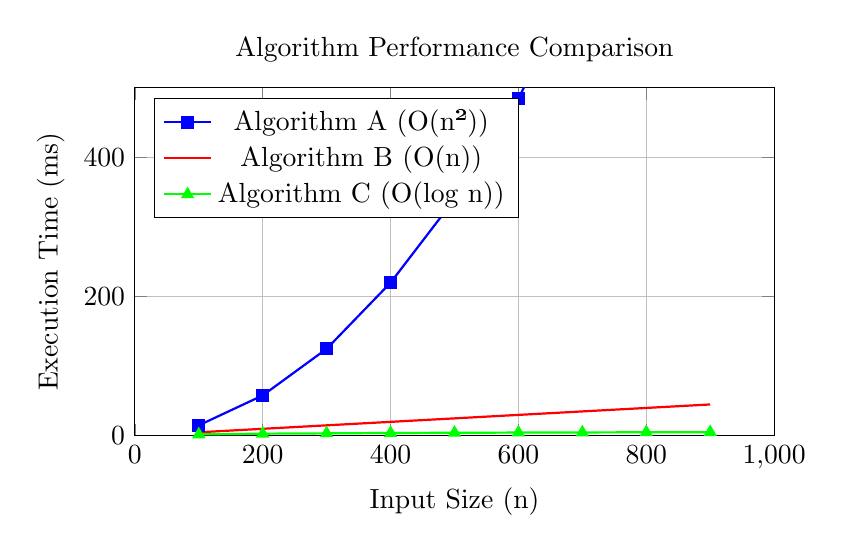
\begin{tikzpicture}
        \begin{axis}[
                title={Algorithm Performance Comparison},
                xlabel={Input Size (n)},
                ylabel={Execution Time (ms)},
                width=0.8\textwidth,
                height=6cm,
                grid=major,
                legend pos=north west,
                xmin=0, xmax=1000,
                ymin=0, ymax=500
            ]

            % Algorithm A - Quadratic complexity
            \addplot[color=blue, mark=square*, thick] coordinates {
                    (100, 15)
                    (200, 58)
                    (300, 125)
                    (400, 220)
                    (500, 340)
                    (600, 485)
                    (700, 665)
                    (800, 875)
                    (900, 1115)
                };
            \addlegendentry{Algorithm A (O(n²))}

            % Algorithm B - Linear complexity
            \addplot[color=red, mark=circle*, thick] coordinates {
                    (100, 5)
                    (200, 10)
                    (300, 15)
                    (400, 20)
                    (500, 25)
                    (600, 30)
                    (700, 35)
                    (800, 40)
                    (900, 45)
                };
            \addlegendentry{Algorithm B (O(n))}

            % Algorithm C - Logarithmic complexity
            \addplot[color=green, mark=triangle*, thick] coordinates {
                    (100, 2)
                    (200, 3)
                    (300, 3.5)
                    (400, 4)
                    (500, 4.3)
                    (600, 4.6)
                    (700, 4.8)
                    (800, 5)
                    (900, 5.2)
                };
            \addlegendentry{Algorithm C (O(log n))}

        \end{axis}
    \end{tikzpicture}
    \caption{Performance comparison showing different algorithmic complexities. Algorithm C demonstrates the best scalability with logarithmic growth, while Algorithm A shows quadratic growth limiting its use for large datasets.}
    \label{fig:performance_comparison}
\end{figure}
